\chapter{Literature Review}
\label{Literature Review}

This chapter builds upon the topics covered in the background by reviewing relevant academic literature. The development and features of the online sports betting industry are first described, followed by an investigation into how machine learning is used for sports prediction. The specific machine learning techniques used in the literature are researched to better understand how they can be used for Counter-Strike match prediction. Additionally, various rating systems used in sports and esports are identified and discussed. The chapter concludes with a discussion of predictive analysis in esports. 

\section{The evolution of online sports betting}

Technological advances have caused major shifts in gambling practices over the last two decades. The modern sports betting industry utilizes software engineering, data analysis, and real-time processing to satisfy a rapidly growing market of bettors. Bets are overwhelmingly made through the use of a smartphone app or website, where algorithms are used to set and dynamically update betting odds \cite{inplay}. Prior to this revolution, bets would need to be made either in-person or with an operator over the telephone. Bookmakers would employ teams of statisticians, known as odds compilers, whose job was to spectate sports events or horse races, break them down into fundamental inputs, and calculate probabilities from those inputs. Most statistical odds compiling was done by counting the occurrences of a given event. The development of in-play betting caused a shift towards mathematical modelling for odds compilation, as humans could simply not keep up with multiple simultaneous events unfolding: "\textit{Bookmakers needed automation, which meant models}" \cite{oddscompiler}.

Betfair were one of the pioneers in the industry, leveraging technology to offer a superior value proposition to bettors in the form of a peer-to-peer betting exchange. The platform was first developed in 1998 by programmer and professional gambler Andrew Black, whose original idea was to create a betting system which operated like the US stock exchange. By late 2004, Betfair had over 300 000 customers and saw over GBP 50 million revenue per week. A 2005 study on Betfair's competitive advantage cited Moore's Law, Metcalfe's Law of Networks, and the internet as key enablers of its success. \cite{betfair}.

A betting exchange works by offering two types of bets: 'back' and 'lay', where a 'back' is a conventional bet on an outcome to occur, and a 'lay' is betting \textit{against} the outcome happening. Odds are set by the bettors themselves, with a bet only going through if another participant bet on the 'lay'. In this way, no odds compilation is necessary as odds are driven purely by market forces. The exchange operator generates revenue from a much smaller commissions when compared to traditional bookmakers \cite{bettingexchange}.

Another sports betting platform called EmpireBet was the focus of a recent study into sports betting through the lens of software engineering. The authors noted that the biggest drivers of evolution were advances in connectivity, the transition from trained operators to user-friendly interfaces accessible by anyone, the automation of risk management and administration tasks, integration with cloud computing services, and the adoption of third-party libraries for rapid development \cite{empirebet}.

In-play sports betting features, also known as live betting, have been a driver of growth in the industry. This is because bettors can place multiple bets during a single sports event. Many bookmakers now also offer a 'cash-out' feature, which was first introduced to the market by William Hill in 2012 \cite{inplay}. This feature allows bettors to "take profit early" if the outcome you bet on has become more likely, or to gain a fraction of your wager back if it is becoming more unlikely.

As discussed in Section \ref{background-bet}, another driver of growth in the sports betting industry is the development of esports betting \cite{esportsgambling}. Business Research Insights reported the market size as \$ 9.75 billion US in 2021, and projected it to grow to \$ 35.57 billion US by 2023: a CAGR of 13.7\% \cite{esports-betting-market-report}.

\section{Machine learning for sports prediction}

Over the past two decades, there has been a significant growth in the amount of data collected during sports matches, both structured and unstructured. It is no surprise that machine learning algorithms have become increasingly popular for analysis of these increasingly large and complex datasets \cite{mlsports}. 

Statistical prediction of sports outcomes, such as the match winner or final score, is of great interest to spectators, teams, and other industry stakeholders. In 2020, Horvat and Job analysed 38 research papers aimed at this particular application for various team sports, ranging from basketball, football, cricket, baseball, and American football \cite{mlsports}. They found that feature selection was critical for building effective models. Noting that earlier studies relied solely on expert opinions, newer studies could achieve better results using statistical techniques (such as regularization) for feature selection. 

The machine learning models employed by researchers differed depending on the nature of the data and the complexity of the problem. In most of the studies, multiple supervised learning classification models were trained and compared. These included logistic regression, support vector machines, decision trees \& random forests, Naive-Bayes, and gradient boosting. Neural networks (NN) were the most popular technique used for prediction, as they can effectively model non-linear relationships by capturing complex patterns in the data \cite{nnoverview}. 

The models were all trained using either a chronological segmentation of the dataset, or by using k-fold cross validation. The most common way of measuring performance was using classification accuracy. The researchers found significant variance in the performance of the models depending on the sport, the quality of the data, and the feature selection process used. Figure \ref{fig:mlsports} shows the distribution of maximum classification accuracy achieved in the 38 different papers \cite{mlsports}.

\begin{figure}[h]
	\centering
	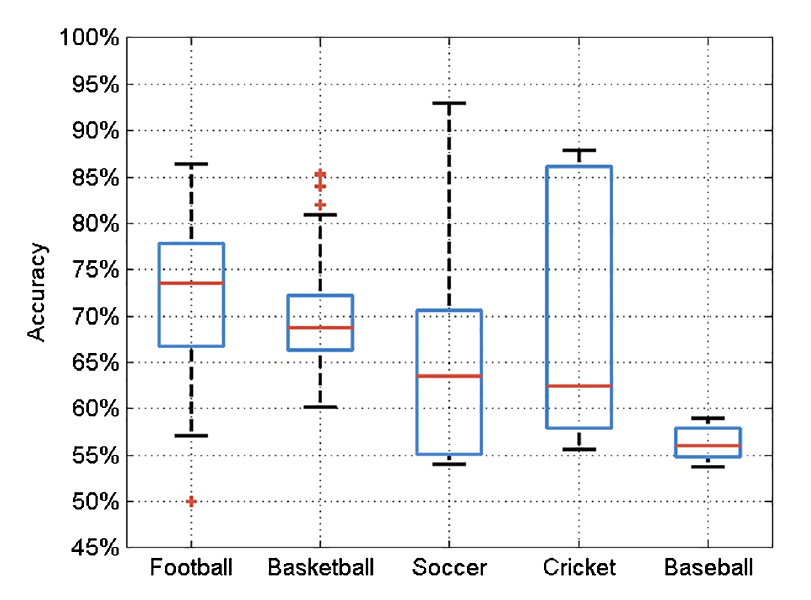
\includegraphics[width=0.8\textwidth]{Figures/mlsports.png}
	\caption{A boxplot of maximum classification accuracies achieved for different sports \cite{mlsports}}
	\label{fig:mlsports}
\end{figure}

Do the same findings apply to esports analysis? Jenny et al. \cite{def-esports} compared esports to traditional sports and argued that, other than the degree of physicality involved, esports display the same characteristics of traditional sports: esports are a voluntary and intrinsically motivated activity, governed by rules, in which opposing players compete. Furthermore, they require skills such as strategic thinking, hand-eye coordination, and rapid decision-making. They concede that the degree of physicality differs significantly, as esports involve fine motor skills as opposed to the high levels of physical exertion typically required in traditional sports. Their research also argued that esports have a global following and are becoming increasingly institutionalized, further cementing their legitimacy. It is therefore reasonable to assume that the techniques described in \cite{mlsports} should, to some extent, be applicable to esports as well. 

\subsection{Machine Learning Algorithms}

In this section the techniques used in the aforementioned papers are investigated. The algorithms include logistic regression, random forests, support vector machines, $k$-nearest neighbours, Naive Bayes, neural networks, and gradient boosting.

\subsubsection{Logistic regression}

Logistic regression (LR) \cite{logreg} is a binary classification algorithm: given an input vector $\bm{x_i}$, classify the output label $y_i$ as 0 or 1. The output value is determined by mapping a linear combination of input values onto the logistic function. This produces a probability $p(\bm{x_i})$ of a given input vector $\bm{x_i}$ (set of features) belonging to the default output class, $y_i = 1$. 

\begin{equation}
p(\bm{x_i}) = \frac{e^{\beta_0 + \beta_1x_{i1} + \beta_2x_{i2} + \ldots}}{1 + e^{\beta_0 + \beta_1x_{i1} + \beta_2x_{i2} + \ldots}} 
\end{equation}

The optimal set of regression coefficients, ${\beta_0, \beta_1, ..., \beta_n}$, is obtained by maximizing the likelihood function. In LR, the likelihood function is the product of the probabilities $p_i$ of each data point being correctly classified by the model. 

\begin{equation}
	\mathcal{L}(\beta_0, \beta_1, ..., \beta_n | y, X) = \prod_{i=1}^{N} p(y_i | \bm{x_i}, \beta_0, \beta_1, ..., \beta_n)^{y_i} \left(1 - p(y_i | \bm{x_i}, \beta_0, \beta_1, ..., \beta_n)\right)^{1 - y_i}
\end{equation}

where $\mathcal{L}$ is the likelihood function, $y_i$ is the actual label of the $i$-th sample, $\bm{x_i}$ is the feature vector of the $i$-th sample, $\beta_0, \beta_1, ..., \beta_n$ are the regression coefficients, and $p(y_i | \bm{x_i}, \beta_0, \beta_1, ..., \beta_n)$ is the predicted probability of the $i$-th sample belonging to the positive class given the feature vector and coefficients.

Because maximizing the likelihood function is computationally challenging, the negative log-likelihood (also known as cross-entropy loss) function is minimized instead. For logistic regression, the loss function is defined as:

\begin{equation}
L(y, p) = -\frac{1}{N} \sum_{i=1}^{N} \left[ y_i \log(p_i) + (1 - y_i) \log(1 - p_i) \right]
\end{equation}

where $L(y, p)$ is the loss function, $N$ is the number of samples, $y_i$ is the actual label, and $p_i$ is the predicted probability that the $i$-th sample belongs to the positive class.

This is an optimization process which is performed iteratively. The logistic regression model therefore fits a logistic curve (also known as a sigmoid) to the data, such that the set of regression coefficients used minimizes the cross-entropy loss function. LR is most appropriate when the class distribution is balanced and a linear relationship exists between the input variables and the output class.

\subsubsection{Decision trees and random forests}

A decision tree resembles a flowchart-structure with three elements: internal nodes which represent different split points on features, branches which represent decision rules, and leaf nodes which represent the outcome. Starting at the top-most node (root), the decision tree is recursively partitioned into progressively smaller sub-trees. 

There are multiple methods for determining the splitting criterion at each node, such as Information gain (the difference in entropy before and after a split) and Gini impurity. The latter quantifies the 'purity' of a node, with lower values representing more homogenous nodes. The Gini Impurity for a single node is calculated using the following formula, where $p_i$ is the probability of an observation being classified into the $i^{th}$ class.

\begin{equation}
Gini\, Impurity = 1 - \sum (p_i)^2
\end{equation}

As an objective function for determining splits, the Gini Impurity is calculated across all leaf nodes. The split that results in the greatest reduction in weighted average impurity across the child nodes is then performed. 

The depth of a decision tree affects its performance and complexity. More complex relationships can be modelled by deeper trees, but these are also more prone to overfitting. 

Overfitting can be mitigated using several techniques. Decision trees can be pruned back according to a cross-validated cost complexity criterion. Their maximum depth can be limited, which prevents them from becoming too complex. The minimum number of samples required to split an internal node can be increased, ensuring that there is enough data to make a decision.

Random forests \cite{randomforests} is an ensemble model; it combines the outputs of many, simpler decision trees which are each trained on a different random subset of the dataset. This technique is known as bagging and it helps to prevent models from over-fitting the training data. Random forests are typically more robust and have an improved accuracy when compared to a single decision tree. 

\subsubsection{Support vector machines}

A support vector machine (SVM) \cite{svm} is classification model which aims to separate data points into their output classes by means of a \textit{hyperplane}. The \textit{margin} is the distance between the hyperplane and the nearest data point in each class. A SVM aims to maximize the margin as far as possible. If a linear hyperplane cannot separate the data well enough, the data can transformed into a higher-dimensional space using a \textit{kernel} function.

A hyperplane in an \( n \)-dimensional space can be defined as:
\begin{equation}
	\mathbf{w} \cdot \mathbf{x} + b = 0
\end{equation}
where \( \mathbf{w} \) is the normal vector to the hyperplane, \( \mathbf{x} \) is a data point, and \( b \) is the bias term.

The margin, which SVMs aim to maximise, is the distance between the hyperplane and the nearest data point from either class. The points lying on the margin boundaries are called support vectors. The distance from a point \( \mathbf{x}_i \) to the hyperplane is given by:
\begin{equation}
	\frac{|\mathbf{w} \cdot \mathbf{x}_i + b|}{\|\mathbf{w}\|}
\end{equation}

For a binary classification problem with labels \( y_i \in \{ -1, 1 \} \), the optimisation problem to maximise the margin can be formulated as:
\begin{equation}
	\begin{aligned}
		& \min_{\mathbf{w}, b} \quad \frac{1}{2} \|\mathbf{w}\|^2 \\
		& \text{subject to} \quad y_i (\mathbf{w} \cdot \mathbf{x}_i + b) \geq 1, \quad \forall i
	\end{aligned}
\end{equation}

As mentioned before, when the data is not linearly separable, SVMs use a \textit{kernel} function to map the input features into a higher-dimensional space where a linear hyperplane can be used to separate the data. Commonly used kernel functions include a \textit{linear} kernel, a \textit{polynomial} kernel, or a \textit{radial basis function} (RBF) kernel. A graphical representation of the effect of using a kernel function is shown in Figure \ref{fig:svm}.

\begin{figure}[h]
	\centering
	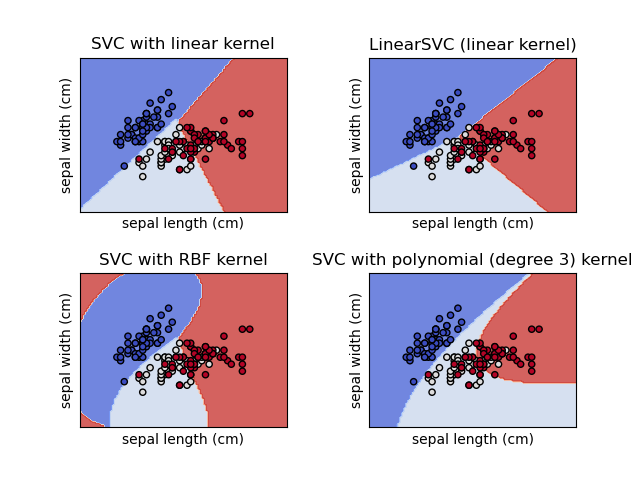
\includegraphics[width=\textwidth]{Figures/svm.png}
	\caption{Hyperplanes for a SVM using different kernel functions \cite{scikitsvm}}
	\label{fig:svm}
\end{figure}

When using a kernel function, the optimization problem becomes:
\begin{equation}
	\begin{aligned}
		& \min_{\mathbf{w}, b, \xi} \quad \frac{1}{2} \|\mathbf{w}\|^2 + C \sum_{i=1}^{n} \xi_i \\
		& \text{subject to} \quad y_i (\mathbf{w} \cdot \phi(\mathbf{x}_i) + b) \geq 1 - \xi_i, \quad \xi_i \geq 0, \quad \forall i
	\end{aligned}
\end{equation}
where \( \phi(\mathbf{x}) \) is the mapping to the higher-dimensional space, \( \xi_i \) are slack variables allowing for misclassification, and \( C \) is a regularisation parameter balancing margin maximization and classification error.

\subsubsection{\textit{k}-nearest neighbours}

$k$-nearest neighbours ($k$-NN) \cite{knn} is a simple algorithm that classifies new observations into the majority class among its nearest neighbouring observations in the feature space. Given an input vector \( \mathbf{x}_i \), the class label \( y_i \) is predicted by the most frequent class among the \( k \) closest neighbours in the training set.

For a new data point \( \mathbf{x}_i \), the predicted class \( \hat{y}_i \) is determined by:
\begin{equation}
	\hat{y}_i = \arg\max_{y} \sum_{\mathbf{x}_j \in N_k(\mathbf{x}_i)} I(y_j = y)
\end{equation}
where \( N_k(\mathbf{x}_i) \) is the set of \( k \) nearest neighbors of \( \mathbf{x}_i \), and \( I(\cdot) \) is the indicator function.

Using a smaller \( k \) value makes the model more sensitive to noise, while a larger \( k \) value may smooth over useful patterns.

The distance between data points \( \mathbf{x}_i \) and \( \mathbf{x}_j \) is usually measured using the Euclidean distance:
\begin{equation}
	d(\mathbf{x}_i, \mathbf{x}_j) = \sqrt{\sum_{m=1}^{M} (x_{im} - x_{jm})^2}
\end{equation}
where \( M \) is the number of features. Note that other measures of distance, such as Manhattan or Minkowski, can also be used.

$k$-NN differs from other models in that there is no training phase, however it can be computationally expensive during the testing phase and is often sensitive to irrelevant features.

\subsubsection{Naive Bayes}

Naive Bayes \cite{gaussiannb} is a probabilistic classifier based on Bayes' theorem. Bayes' theorem quantifies the probability of an event occurring given prior knowledge of the conditions related to the event. 

\begin{equation}
	P(A|B) = \frac{P(B|A) \cdot P(A)}{P(B)}
\end{equation}

where $P(A|B)$ is the conditional probability of event A occurring given that event B is true, and $P(A)$ and $P(B)$ are the independent probabilities of event A or B occurring.

It is "naive" as it assumes that the predictors (features) are conditionally independent given the class, i.e. the presence (or absence) of a particular feature in a class is unrelated to the presence (or absence) of any other feature in that class.

The Gaussian Naive Bayes classifier is a Naive Bayes algorithm which assumes that all continuous features are normally distributed. The probability of a feature value given a class is thus calculated using the Gaussian probability density function.

For a new data point \( \mathbf{x}_i \), the predicted class \( \hat{y}_i \) is determined by:
\begin{equation}
	\hat{y}_i = \arg\max_{y} p(y) \prod_{j=1}^{n} p(x_{ij} | y),
\end{equation}
where \( p(y) \) is the prior probability of class \( y \), and \( p(x_{ij} | y) \) is the conditional probability of feature \( j \) given class \( y \), assumed to be Gaussian:
\begin{equation}
	p(x_{ij} | y) = \frac{1}{\sqrt{2\pi\sigma_{yj}^2}} \exp\left( -\frac{(x_{ij} - \mu_{yj})^2}{2\sigma_{yj}^2} \right),
\end{equation}
where \( \mu_{yj} \) and \( \sigma_{yj}^2 \) are the mean and variance of feature \( j \) in class \( y \), respectively.

\subsubsection{Neural networks}

A neural network (NN)  \cite{mlp} consists of many densely interconnected nodes. In a feed-forward network, data moves in one direction only - forward. It traverses the network from the input layer, through multiple hidden layers of nodes, to an output layer. Figure \ref{fig:feedforward} is an example of this structure. 

Each node assigns a weight to its incoming connections, and emits an output using an activation function. This function computes an output from each weighted input and a threshold value. During training, the weights and thresholds are adjusted until convergence \cite{nnoverview}. At convergence, these values stabilize and do not change significantly with further training.

\begin{figure}[h]
	\centering
	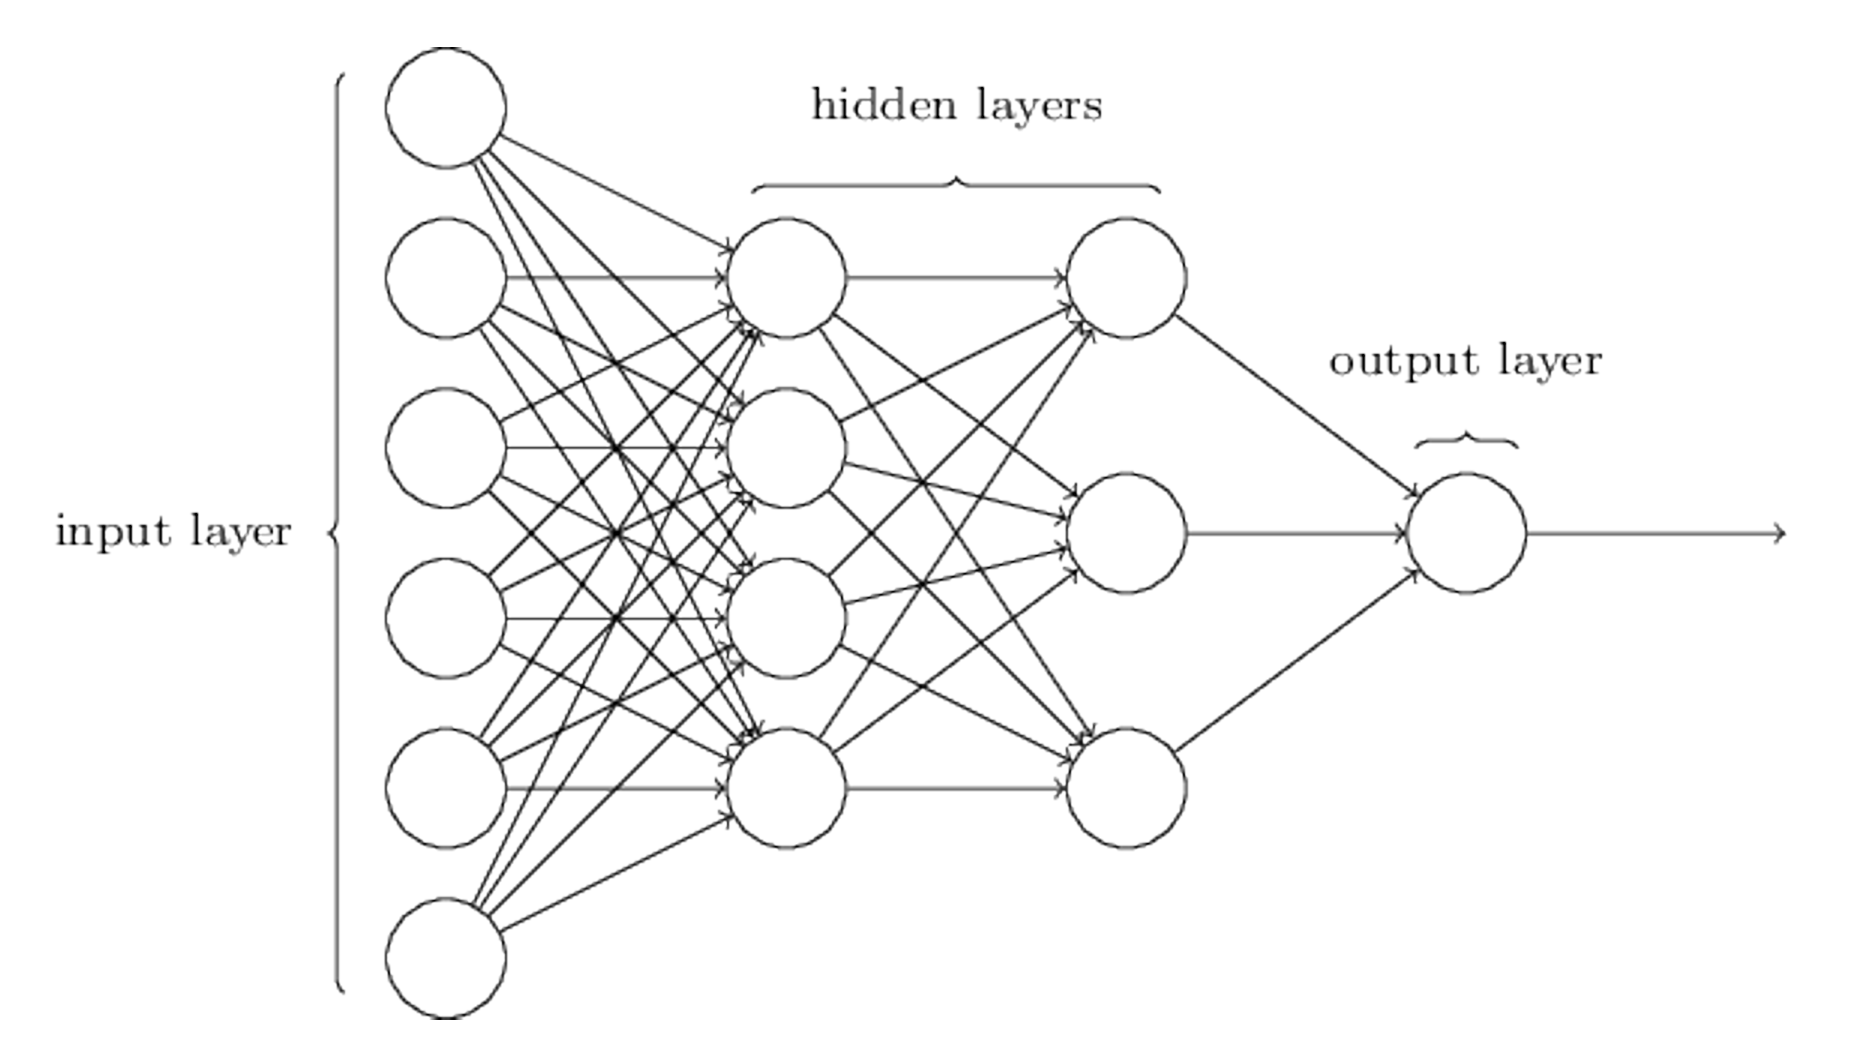
\includegraphics[width=0.8\textwidth]{Figures/feedforward.png}
	\caption{A simple feed-forward neural network \cite{nn_fig}}
	\label{fig:feedforward}
\end{figure}

They key parameters which affect the network's capacity to model complex relationships in the data are the depth of the network (the number of hidden layers), the width (the number of nodes in each hidden layer), and the activation function used in the hidden layers. Common activation functions include 

\begin{itemize}
	\item Rectified Linear Unit (ReLU)
	\begin{equation}
		f(x) = \max(0, x)
	\end{equation}
	where \( f(x) \) is the activation function applied to the input \( x \) of a neuron.
	
	\item Sigmoid
	\begin{equation}
		\sigma(x) = \frac{1}{1 + e^{-x}}
	\end{equation}
	Sigmoid squashes the output to the range [0, 1], which is useful for binary classification tasks.
	
	\item Tanh (Hyperbolic tangent)
	\begin{equation}
		\tanh(x) = \frac{e^x - e^{-x}}{e^x + e^{-x}}
	\end{equation}
	Tanh squashes the output to the range [-1, 1], which helps with zero-centered data and mitigates the vanishing gradient problem.
\end{itemize}

The activation function used impacts the training and performance of the NN. ReLU is commonly used in hidden layers due to its simplicity and effectiveness in training deep networks, while sigmoid and tanh are used in the output layer for binary classification.

There are multiple types of neural networks with different applications. Feed-forward neural networks, such as multilayer perceptrons (MLPs), work as described above. MLPs consist of at least three layers of nodes and can be used for both classification and regression tasks. 

Recurrent neural networks (RNNs) are designed for sequential data processing. They have connections that form directed cycles, thereby maintaining a hidden state that can capture information from previous time steps. The hidden state is updated iteratively using the current input and the previous hidden state. This feedback loop makes RNNs suitable for tasks involving time series data and natural language processing.

Convolutional neural networks (CNNs) are designed to process data with a grid-like topology, such as images. They consist of one or more convolutional layers, where each layer applies convolutional filters to small regions of the input, capturing local patterns and spatial hierarchies. This makes CNNs suitable for tasks like image recognition \cite{cnn-paper}.

\subsubsection{Gradient boosting}

Gradient boosting \cite{friedmanboosting} is an ensemble technique that differs from random forests in that each tree is built sequentially, where each new tree is trained to 'correct' the errors of the previously trained trees. 

The process begins with an initial model, typically a simple predictor, such as the mean of the target values for regression problems. With each iteration, the pseudo-residuals (the difference between the predicted and actual values) are calculated and the subsequent tree is built to predict these residuals. The model is updated by adding the predictions from this tree, weighted by a learning rate $\lambda$, to the initial predictions. This iterative fine-tuning process is repeated until convergence or another stopping criterion is met. 

This process is mathematically formulated as follows:

The \textbf{initial model} \( F_0(x) \) is chosen to minimize the loss function over all training examples.
\begin{equation}
	F_0(x) = \arg\min_{\gamma} \sum_{i=1}^{n} L(y_i, \gamma)
\end{equation}
where \( L(y, \hat{y}) \) is the loss function, \( y_i \) is the actual value, and \( \gamma \) is a constant (e.g., the mean of \( y \) for regression).

For each \textbf{iteration}, \( m = 1 \) to \( M \) (the total number of iterations):

(a) Compute the pseudo-residuals:
\begin{equation}
	r_i^{(m)} = -\left[\frac{\partial L(y_i, F_{m-1}(x_i))}{\partial F_{m-1}(x_i)}\right]
\end{equation}
These residuals represent the gradient of the loss function with respect to the current model's predictions.

(b) Fit a base learner (e.g., a decision tree) \( h_m(x) \) to the pseudo-residuals:
\begin{equation}
	h_m(x) \approx r_i^{(m)}
\end{equation}

(c) The optimal step size \( \gamma_m \) is computed to minimize the loss function after adding the new learner's predictions:
\begin{equation}
	\gamma_m = \arg\min_{\gamma} \sum_{i=1}^{n} L(y_i, F_{m-1}(x_i) + \gamma h_m(x_i))
\end{equation}

(d) Update the model by adding the scaled predictions of the new learner to the current model
\begin{equation}
	F_m(x) = F_{m-1}(x) + \lambda \gamma_m h_m(x)
\end{equation}
where \( \lambda \) is the learning rate.

After \( M \) iterations, the \textbf{final model} is given by:
\begin{equation}
	F_M(x) = F_0(x) + \sum_{m=1}^{M} \lambda \gamma_m h_m(x)
\end{equation}

XGBoost (eXtreme Gradient Boosting) \cite{xgboost} is an advanced, scalable implementation of gradient boosting which regularly outperforms other models for classification tasks \cite{gradboostingwins}. It introduces a number of improvements over gradient boosting:

XGBoost uses a second-order Taylor approximation of the loss function $L$ to make the optimization problem more accurate. Regularisation is introduced into the objective function which penalises model complexity, thereby reducing overfitting. It handles sparse and missing data efficiently using a sparsity-aware split finding algorithm. Furthermore, tree construction is parallelised for enhanced computational efficiency.

\subsection{Rating systems}

Ratings and ranks serve as indicators of the relative performance of players or teams. These indicators are determined using different methods that vary from sport to sport, however they are always modelled on prior data. The ratings then serve as predictors for future data, and there is an implicit expectation that higher-rated teams are expected to beat lower-rated teams more often than not. A good rating system is one which represents the true skill level as accurately as possible. This section investigates the Elo, Glicko, and TrueSkill rating systems.

\subsubsection{Elo}
\label{elo}

The Elo rating system was developed by Hungarian-American physics professor Arpad Elo \cite{elo}. Its original purpose was to rank the strength of different chess players, however it can be applied to any zero-sum game. The Elo system has been used to rate teams and players in many other sports, including football, baseball, and esports. The central idea is that the difference between two players' Elo ratings serves as a predictor of the match outcome. Each player's Elo rating is a single value, $R$. After each game, the winner gains points and the loser loses points. The magnitude of the loss and gain is different for each player, depending on their original Elo ratings. A mathematical description of the Elo rating system follows. 

Let players A and B have initial ratings $R_A = 900$ and $R_B = 1000$. The expected score for player A and B is given by the logistic function with base 10:

\[ E_A = \frac{1}{1 + 10^{(R_B - R_A) / 400}} = 0.360 \]
\[ E_B = \frac{1}{1 + 10^{(R_A - R_B) / 400}} = 0.640 \]

As shown above, the expected outcomes are complements of each other, adding up to $1$. After the match is played, the player ratings are then updated:

\[ R_A^{'} = R_A + K \cdot (S_A - E_A) \]

where $S_A$ is the actual score for player A and $K$ is the maximum possible adjustment per game. Adjusting the $K$-factor will adjust the sensitivity of the system to change. Assuming that player A won the game, $S_A = 1$, and $K = 50$,

\[ R_A^{'} = 800 + 50 \cdot (1 - 0.360) \approx 932 \]
\[ R_B^{'} = 1000 + 50 \cdot (0 - 0.640) \approx 968 \]

Player A's Elo rating has increased, and Player B's has decreased. If the players were to play another game, the expected outcome has now changed to reflect their new ratings:

\[ E_A^{'} = 0.448 \]
\[ E_B^{'} = 0.552 \]

In this way, all players can be rated on the same scale and the probability of winning is easily calculated. In the graph in Figure \ref{fig:elo}, the expected score can be interpreted as the probability of the first player winning. For example, as the difference in Elo rating approaches 800, the probability of the player with the higher Elo rating winning approaches 100\%.

\begin{figure}[h]
	\centering
	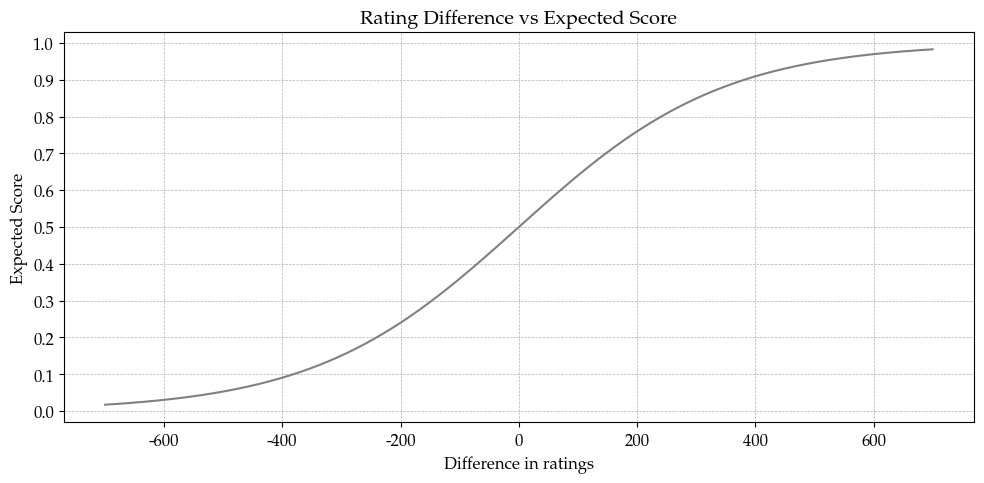
\includegraphics[width=\textwidth]{Figures/elo.png}
	\caption{Difference in player Elo ratings vs expected score}
	\label{fig:elo}
\end{figure}

\subsubsection{Glicko}

In practice, the $K$-factor used in the Elo system is not always held constant. For example, when trying to rank new players, it is sensible to allow their ratings to change rapidly, and decrease $K$ over time, as more games are played and more becomes known about their skill level. The 'Glicko' system, created in 1995 by Mark Glickman \cite{glicko}, introduces the concept of a \textit{Ratings Deviation} (RD), or standard deviation, to account for the uncertainty of a player's rating. A low RD indicates a higher level of certainty about the player's rating, whereas a high RD is typical for players who compete infrequently or only have a few games played.

A central idea to the Glicko system is the \textit{rating period}. Ratings and RD are determined for each player at the start of a new rating period:

\[
RD = \min \left\{ \sqrt{RD_0^2 + c^2t}, 350 \right\}
\]

The expected score for player A against player B is then given by:
\[
E_A = \frac{1}{1 + 10^{g(RD_B) \cdot (R_B - R_A) / 400}}
\]
where \( g(RD) \) is a function that scales the influence of the rating deviation.

The updated rating and rating deviation for player A after a series of games is calculated as:
\[
R_A' = R_A + \frac{q}{(1/RD_A^2) + (1/d^2)} \sum_{i=1}^{n} g(RD_i)(S_i - E_i)
\]
\[
RD_A' = \sqrt{\left(\frac{1}{RD_A^2} + \frac{1}{d^2}\right)^{-1}}
\]
where \( q \) is a constant, \( d^2 \) is a term derived from the expected scores and outcomes of the games played, and \( n \) is the number of games played in the rating period.

In contrast to the Elo system where both players' ratings change by the same magnitude, in the Glicko system this amount is governed by their opponent's RD.

\subsubsection{TrueSkill\texttrademark}

TrueSkill\texttrademark{} is a skill rating system designed by Microsoft Research and published in January 2007 \cite{trueskill}. TrueSkill was designed specifically for multiplayer online games, with the intention of matching players together with similar skill levels such that the games were more "enjoyable, fair, and exciting". Each player's skill level is modelled as a Gaussian distribution, $\mathcal{N}(\mu, \sigma^2)$, where $\sigma^2$ is the variance of the distribution, and a smaller value reflects higher confidence in the player's skill level $\mu$.

New players start with a default skill distribution. After each match, Bayesian inference is used to update and predict players' skill levels, using pairwise comparisons between each player in each team. These comparisons are evaluated using the cumulative distribution function of the difference of two players' TrueSkill ratings, which is also a Gaussian. The expected probability of player A beating player B can therefore be calculated as:
\[P(A \text{ beats } B) = \Phi\left(\frac{\mu_A - \mu_B}{\sqrt{\sigma_A^2 + \sigma_B^2}}\right)\]
where ($\Phi$) is the cumulative density function of the standard normal distribution, ($\mu_A$) and ($\mu_B$) are the skill estimates of players A and B respectively, and ($\sigma_A$) and ($\sigma_B$) are their corresponding uncertainties.

Over time and with more games played, the standard deviation $\sigma$ of a player's skill distribution decreases, reflecting increased confidence in their skill level estimation.

TrueSkill\texttrademark{} expands upon the foundations of Elo and Glicko, with key advances being the ability to rate each individual in a team of players, and allowing for matches of more than two players or teams to to be modelled. For team games, TrueSkill treats the team's skill as the sum of the skills of its members. In their research paper, Herbrich et al.  \cite{trueskill} demonstrated that TrueSkill worked well in their experiments with hundreds of thousands of Xbox Live players.

\section{Predictive analysis in esports}

Esports have the unique characteristic of being natively digital. This means that recording data from a given match is much cheaper and easier than traditional sports, and even amateur games can be recorded in fine detail. In the age of \textit{big data}, esports are therefore well-positioned for data analysis. 

This is reflected by the significant number of papers that have been written on the topic of prediction in different esports, with a particular emphasis on real-time match analysis. Hodge et al. \cite{livematchprediction} performed a comprehensive case study on live win prediction in Dota~2, and concluded that win prediction is difficult, where no single technique excels. They suggested combining techniques into ensembles to achieve better performance. These events were combined with pre-game information to construct the feature set. The ML algorithms used were logistic regression, random forests, and LightGBM, a performant gradient-boosting algorithm. They found that LightGBM outperformed both logistic regression and random forest. Dota~2 matches last 40 minutes on average but can be as short as 10 minutes. Noting a shortage of professional matches to use for analysis, their approach was to use an input data set of 5744 game replays from highly rated, but not necessarily professional players. The dataset was chronologically split, with two-thirds for training and the remainder for testing. They further tested their models on a significantly smaller set of 186 tournament matches. Despite a poor pre-match prediction accuracy of 55.8\%, they found that when using features known 20 minutes into the game (the average half-way point of a match) they could predict the winner of professional games with 74.59\% accuracy.

A similar study was conducted by Yang et al. \cite{yang2016realtime}, with an expanded dataset of 78263 Dota~2 matches. By considering player history, they could improve the pre-match feature set. This allowed the authors to achieve a 71.49\% accuracy using logistic regression and 70.46\% using neural networks. With live prediction, they found that a key factor affecting performance was the time of the match, with real-time features becoming increasingly informative as the match progresses. At the 40th minute of the match, their model achieved 93.73\% prediction accuracy.

A number of studies have been done on different aspects of Counter-Strike gameplay. Bednárek et al. \cite{demofileprocessing} described how to accurately parse data from demo files, which often contained inconsistencies or errors. They also described how player identities could be linked from the demo files to their online player profiles. The extracted demo-file data is ripe for live feature generation; Marshall et al. \cite{livedeaths} used convolutional and recurrent neural networks to predict the probability of a player dying within the next 5 seconds. The input features were recorded from 542 matches, with 5 second windows of information containing features related to damage events. They found long short-term memory, a form of recurrent neural network, yielded the best performance.

Xenopolous et al. \cite{wpacs} created a framework, known as 'Win Probability Added', for valuing individual player contributions to their team's round-win percentage. They extracted over 70 million data points from 4682 demo files. Their research employed machine learning models such as logistic regression and gradient boosting (CatBoost and XGBoost) to generate the win probabilities. Another study \cite{spendingerror} focused on modelling 'Optimal Economic Decisions' for a given round in CS. This study employed XGBoost and neural networks on a dataset derived from 6538 demo files. They found a correlation between spending errors and lower round win-rates.

Some research has been done in pre-match CS win prediction. Švec \cite{svec} used online match data to train machine learning models to predict match winners. They achieved 60\% classification accuracy using graph convolutional networks, which was "disappointing" when compared to the performance attained with a comparatively simple Elo-based baseline prediction. Another study \cite{mapvetoml} aimed to create a decision support system to estimate the win probability for a given map. The researchers trained a linear regression and random forests model with player data from FACEIT, a popular third-party match-making service. They managed to attain an overall match prediction accuracy of 57.42\%. A similar study \cite{faceitclusters} used k-means to cluster players together using data from their FACEIT matches. Once clustered, the player data was used to train a feed-forward neural network to determine their win probability. An accuracy of 65.11\% was obtained, which exceeded their benchmark prediction made from win-rates alone.

\section{Summary}

It is evident that sports prediction using machine learning techniques is a popular field of research. The key factors affecting performance are the quality of data used, the features that can be derived, the choice of ML algorithms, and the sport in question \cite{mlsports}. Unpredictability is an inherent characteristic of sports, and esports are no different.

The studies surrounding Counter-Strike match prediction are noteworthy, however more work can be done to expand upon the results obtained: the quality and quantity of data, as well as the features derived therefrom, can be improved. Furthermore, studies typically measure the performance with respect to statistical metrics, such as classification accuracy, F1-score, and AUC. By expanding the scope of the study to generate betting odds, a comparison with real-world betting odds can be made, which may produce novel and valuable insights into the ever-expanding industry of online sports betting.